\section{Introduction}

Daily stock returns are close to unpredictable in their sign but not in their size: large moves cluster in time. Stochastic volatility (SV) models describe this with a latent log-variance $X_j$ that evolves as a Markov chain and scales the return $R_j$ observed on day $j$. Inferring $X_j$ from the returns $r_{1:j}$ observed so far is a filtering problem in the sense of Chapter 9 of the lecture notes \cite{sanzAlonsoAlGhattas}, with $R_j$ in the role of the observation $Y_j$. The observation depends nonlinearly on the state, and particle filters are the natural tool.

This project studies one modeling choice and its computational consequences: how the shock to the return is correlated with the shock to the volatility. In the classical leverage specification, today's return moves tomorrow's volatility; in the specification of Jacquier, Polson and Rossi \cite{jacquierPolsonRossi2004}, today's return and today's volatility move together. Both are one-parameter extensions of the basic SV model, but they lead to very different particle filters. In the second, the return observed on day $j$ is informative about the volatility shock of day $j$, and the bootstrap particle filter, which proposes that shock blindly, loses most of its effective sample size. A guided proposal derived from the optimal particle filter of Section 9.3 of the notes restores it. The improvement matters beyond filtering: the noise of the particle likelihood biases the simulated maximum likelihood estimate of the correlation.

The data are daily open-to-close log returns of the S\&P 500 from 2000-01-03 to 2021-05-18 (5358 days). Parameters are estimated on 2000--2015 (4015 days), and the models are compared with each other and with GARCH benchmarks by one-step forecasts on the 1343 held-out days from 2016-01-04 on. A 5-minute realized variance (RV) from the Oxford-Man Realized Library \cite{heberEtAl2009} is used to motivate the models and to evaluate forecasts, never for estimation or filtering. The accompanying notebook reproduces every number and figure.

\section{Stochastic Volatility with Return--Volatility Correlation}

\subsection{Three models}

All models in this project share the observation and state equations
\begin{align}
        R_j &= a + e^{X_j/2}\eta_j, \label{eq:obs}\\
        X_{j+1} &= \mu + \phi(X_j - \mu) + \sigma_X \xi_{j+1}, \label{eq:state}
\end{align}
with standard normal shocks $\eta_j$ and $\xi_j$, $|\phi| < 1$, $\sigma_X > 0$, and the stationary initialization $X_0 \sim \Nc(\mu, \sigma_X^2/(1-\phi^2))$. Here $\mu$ is the long-run level of the log-variance, $\phi$ its persistence and $\sigma_X$ the size of its shocks; $e^{X_j/2}$ is the volatility of day $j$. The models differ only in the dependence between the shocks. With parameter $\theta = (a, \mu, \phi, \sigma_X, \rho)$:
\begin{enumerate}[(i)]
        \item \emph{No correlation}: all shocks are independent and $\rho = 0$. This is the basic log-normal SV model \cite{kimShephardChib1998}.
        \item \emph{Next-day correlation}: $\operatorname{corr}(\eta_j, \xi_{j+1}) = \rho$, that is, $\xi_{j+1} = \rho\eta_j + \sqrt{1-\rho^2}\,\zeta_{j+1}$ with $\zeta_{j+1} \sim \Nc(0,1)$ independent of everything else. A negative $\rho$ is the leverage effect: a fall today raises tomorrow's volatility \cite{harveyShephard1996, yu2005, omoriEtAl2007}.
        \item \emph{Same-day correlation}: $\operatorname{corr}(\eta_j, \xi_j) = \rho$ \cite{jacquierPolsonRossi2004}. The shock that moves the volatility of day $j$ also moves the return of day $j$.
\end{enumerate}
In all three models $\xi_{j+1}$ is independent of $X_j$, so $X$ is marginally the same stationary Gaussian AR(1) process, and $\rho = 0$ gives model (i) in either timing. What changes is the conditional structure a filter has to work with. In model (ii) the observation density is that of model (i),
\begin{equation}
        g(r \mid x) = \Nc\big(r;\, a,\, e^{x}\big),
        \label{eq:g_i}
\end{equation}
but the transition depends on the previous return through $\eta_j = (R_j - a)e^{-X_j/2}$:
\begin{equation}
        X_{j+1} \mid X_j, R_j \sim \Nc\Big(\mu + \phi(X_j - \mu) + \rho\sigma_X(R_j - a)e^{-X_j/2},\; (1-\rho^2)\sigma_X^2\Big).
        \label{eq:trans_ii}
\end{equation}
In model (iii) the transition is \eqref{eq:state}, and writing $\eta_j = \rho\xi_j + \sqrt{1-\rho^2}\,\varepsilon_j$ with $\varepsilon_j \sim \Nc(0,1)$,
\begin{equation}
        R_j \mid X_{j-1}, \xi_j \sim \Nc\Big(a + \rho e^{X_j/2}\xi_j,\; (1-\rho^2)e^{X_j}\Big),
        \qquad X_j = \mu + \phi(X_{j-1} - \mu) + \sigma_X\xi_j.
        \label{eq:g_iii}
\end{equation}
With $\rho < 0$, a large $\xi_j$ raises the volatility and lowers the return on the same day, so the one-day predictive distribution of $R_j$ is skewed to the left. In models (i) and (ii) it is symmetric about $a$. Yu \cite{yu2005} argues that only (ii) is leverage in the sense of the continuous-time models it discretizes; we read (iii) simply as a statement about how returns and volatility move within a day.

\subsection{What the data suggest}

Two facts guide these choices; they use RV, which appears nowhere else before the evaluation in Section~\ref{sec:forecasts}. First, returns are far from Gaussian (excess kurtosis 8.4), but returns standardized by the same day's RV are close to Gaussian (excess kurtosis $-0.39$, skewness $0.00$), as documented in \cite{andersenEtAl2001}. We therefore keep $\eta_j$ Gaussian and leave the fat tails to the volatility. Second, the return is correlated with the change of $\log\mathrm{RV}$ on the same day ($-0.195$, and $-0.347$ in 2016--2021) much more strongly than with its change on the next day ($-0.086$, and $+0.049$ in 2016--2021). This is the reason to compare model (iii) with the classical model (ii).

\subsection{Benchmarks}

GARCH(1,1) \cite{bollerslev1986} sets the conditional variance to $h_j = \omega + \alpha\varepsilon_{j-1}^2 + \beta h_{j-1}$ with $\varepsilon_j = r_j - a$ and $R_j \mid r_{1:j-1} \sim \Nc(a, h_j)$. GJR-GARCH \cite{glostenEtAl1993} adds $\gamma\varepsilon_{j-1}^2\mathbb{1}\{\varepsilon_{j-1} < 0\}$ and is the GARCH analogue of model (ii). Their variance is a deterministic function of past returns, so their likelihood is available in closed form and is maximized directly.

\section{Particle Filters for the Three Models}

\subsection{Bootstrap filter and likelihood estimate}

For fixed $\theta$, the filtering densities $f_j$ of $X_j \mid R_{1:j} = r_{1:j}$ obey the prediction--analysis recursion of Section 9.1 of the notes. The bootstrap particle filter of Section 9.2 applies to all three models: in model (ii) the transition \eqref{eq:trans_ii} only involves the known return $r_j$, and in model (iii) the pair $(X_{j-1}, \xi_j)$ determines both $X_j$ and the observation density \eqref{eq:g_iii}. Algorithm~\ref{alg:pf} states the filter with a general proposal $q$ for $\xi_j$ in model (iii); the bootstrap filter uses $q = \Nc(0,1)$.

Besides the filtering means, the filter estimates the likelihood,
\begin{equation}
        \hat L(\theta) = \prod_{j=1}^J \frac1N\sum_{n=1}^N \tilde w_j^{(n)}
        \;\approx\; p_\theta(r_{1:J}) = \prod_{j=1}^J p_\theta(r_j \mid r_{1:j-1}),
        \label{eq:Lhat}
\end{equation}
and $\hat L(\theta)$ is unbiased for every $N$ \cite{delMoral2004, chopinPapaspiliopoulos2020}. Its logarithm is not: if $\log\hat L$ is approximately Gaussian with variance $s^2$, then $\Expect[\log\hat L] \approx \log p_\theta(r_{1:J}) - s^2/2$ \cite{doucetEtAl2015}. This bias matters in Section~\ref{sec:estimation}. Weights are computed on the log scale, and particles are sorted before systematic resampling: with a fixed stream of random numbers, sorting makes $\theta \mapsto \log\hat L(\theta)$ nearly continuous for a one-dimensional state, which helps the optimizer \cite{malikPitt2011}.

\begin{algorithm}[t]
\caption{Particle filter for models (i)--(iii)}
\label{alg:pf}
\begin{algorithmic}[1]
\REQUIRE Returns $r_{1:J}$, parameter $\theta$, number of particles $N$, proposal $q$ (model (iii) only).
\STATE Sample $X_0^{(n)} \sim \Nc\big(\mu, \sigma_X^2/(1-\phi^2)\big)$ for $1 \le n \le N$, and set $\log\hat L = 0$.
\FOR{$j = 1, \dots, J$}
    \FOR{$n = 1, \dots, N$}
        \STATE Set $m^{(n)} = \mu + \phi(X_{j-1}^{(n)} - \mu)$.
        \STATE \emph{Models (i), (ii):} set $\widehat X_j^{(n)} = m^{(n)} + \sigma_X\big(\rho\,\eta^{(n)} + \sqrt{1-\rho^2}\,\zeta^{(n)}\big)$ with $\zeta^{(n)} \sim \Nc(0,1)$ and $\eta^{(n)} = (r_{j-1} - a)e^{-X_{j-1}^{(n)}/2}$ ($\eta^{(n)} = 0$ for $j = 1$; $\rho = 0$ in model (i)), and $\tilde w_j^{(n)} = \Nc\big(r_j;\, a,\, e^{\widehat X_j^{(n)}}\big)$.
        \STATE \emph{Model (iii):} draw $\xi^{(n)} \sim q(\cdot \mid X_{j-1}^{(n)}, r_j)$, set $\widehat X_j^{(n)} = m^{(n)} + \sigma_X\xi^{(n)}$ and
        \[
                \tilde w_j^{(n)} = \Nc\Big(r_j;\, a + \rho e^{\widehat X_j^{(n)}/2}\xi^{(n)},\, (1-\rho^2)e^{\widehat X_j^{(n)}}\Big)\,
                \frac{\Nc(\xi^{(n)}; 0, 1)}{q(\xi^{(n)} \mid X_{j-1}^{(n)}, r_j)}.
        \]
    \ENDFOR
    \STATE Set $\log\hat L \leftarrow \log\hat L + \log\big(N^{-1}\sum_n \tilde w_j^{(n)}\big)$, $w_j^{(n)} = \tilde w_j^{(n)}/\sum_k \tilde w_j^{(k)}$ and $\mathrm{ESS}_j = 1/\sum_n (w_j^{(n)})^2$.
    \STATE Record $\sum_n w_j^{(n)} h\big(\widehat X_j^{(n)}\big) \approx \Expect[h(X_j) \mid r_{1:j}]$.
    \STATE Resample $X_j^{(1)}, \dots, X_j^{(N)}$ from $\sum_n w_j^{(n)}\delta_{\widehat X_j^{(n)}}$ (sorted, systematic).
\ENDFOR
\STATE \textbf{Output:} $\log\hat L(\theta)$, filtering means, $\mathrm{ESS}_{1:J}$.
\end{algorithmic}
\end{algorithm}

\subsection{Why the bootstrap filter degenerates in model (iii)}

In models (i) and (ii) the new state enters the observation density \eqref{eq:g_i} only through the scale, and the bootstrap filter is efficient: at the estimates of Section~\ref{sec:estimation} its average relative ESS, $\mathrm{ESS}_j/N$, is 0.93 and 0.95. In model (iii) the return also carries information about the volatility shock itself. Let $m_j = \mu + \phi(X_{j-1} - \mu)$ and $z_j = (r_j - a)e^{-m_j/2}$. If $\sigma_X$ were zero in the factor $e^{X_j/2}$ of \eqref{eq:g_iii}, the observation would read $z_j = \rho\xi_j + \sqrt{1-\rho^2}\,\varepsilon_j$: a linear Gaussian observation of $\xi_j$ which, at $\rho \approx -0.84$, explains $\rho^2 = 70\%$ of its variance. A bootstrap proposal $\xi_j \sim \Nc(0,1)$ ignores this information, and most particles receive small weights. Figure~\ref{fig:oneday} shows one such day. On 2018-02-05 the index fell by 3.4\% between the open and the close, and given the particles for the previous day the return points to a volatility shock $\xi_j$ near 2.9. The bootstrap proposals lie around zero, and only the few in their upper tail carry weight: the relative ESS is 0.003. Over all days at this parameter, the average relative ESS of the bootstrap filter is 0.52, and it is below 0.1 on 3.5\% of the days (Figure~\ref{fig:pf}, middle).

\begin{figure}[t]
        \centering
        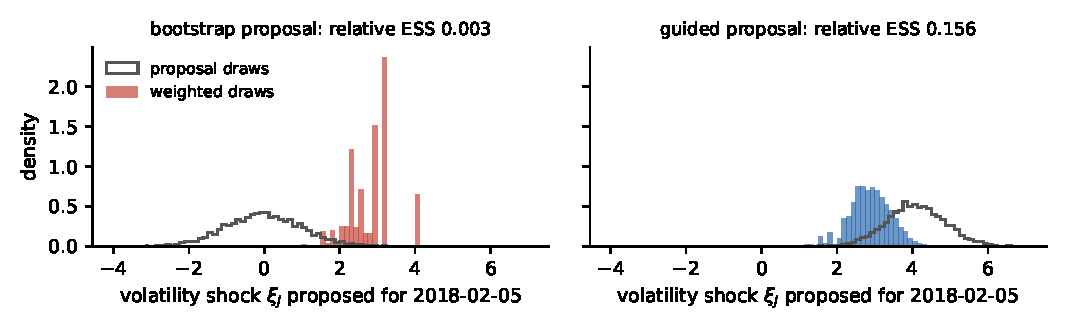
\includegraphics[width=\textwidth]{figures/pf_one_day.pdf}
        \caption{One step of the filter for model (iii) on 2018-02-05, from the same particles for the previous day and with $N = 5000$. Outline: histogram of the proposed volatility shocks $\xi_j^{(n)}$. Filled: the same draws weighted by $w_j^{(n)}$, an approximation of the distribution of $\xi_j$ given $r_{1:j}$.}
        \label{fig:oneday}
\end{figure}

\subsection{A guided proposal from the optimal particle filter}

The optimal particle filter of Section 9.3 of the notes would propose from $P(\xi_j \mid X_{j-1}, R_j)$ and weight by $P(R_j \mid X_{j-1})$. Neither is available in closed form here, because $X_j$ enters \eqref{eq:g_iii} through $e^{X_j/2}$. With $\sigma_X = 0$ in that factor, however, the observation becomes the linear Gaussian one above, which is exactly the setting of Section 9.3 with $H = \rho$, $\Sigma = 1$ and $\Gamma = 1 - \rho^2$: then $S = 1$, the gain is $K = \rho$, and the optimal kernel is $\Nc(\rho z_j, 1 - \rho^2)$. We use this kernel as the proposal,
\begin{equation}
        q(\xi \mid X_{j-1}, r_j) = \Nc\big(\xi;\, \rho z_j,\, 1 - \rho^2\big),
        \label{eq:guided}
\end{equation}
and correct for the approximation through the weights of Algorithm~\ref{alg:pf}. Given a particle $X_{j-1}^{(n)}$, the expected incremental weight under $q$ is
\[
        \int \Nc\Big(r_j;\, a + \rho e^{x(\xi)/2}\xi,\, (1-\rho^2)e^{x(\xi)}\Big)\,\Nc(\xi; 0, 1)\,d\xi = p_\theta\big(r_j \mid X_{j-1}^{(n)}\big),
        \qquad x(\xi) = m_j + \sigma_X\xi,
\]
the same as with the bootstrap proposal. This is the importance sampling identity of Chapter 3 applied particle by particle, and it keeps \eqref{eq:Lhat} unbiased for any proposal whose support contains that of $\Nc(0,1)$. In the terminology of \cite[Chapter 10]{chopinPapaspiliopoulos2020} this is a guided particle filter. As $\sigma_X \to 0$ its weights tend to $\Nc(r_j; a, e^{m_j})$, which depends on $X_{j-1}$ only, as in the optimal filter. The proposal costs one extra exponential per particle and step.

\begin{remark}[Which importance ratio may be used]
The weight of the guided filter contains the ratio $\Nc(\xi; 0, 1)/q(\xi)$. On its own, this ratio has infinite second moment under $q$ whenever $1 - \rho^2 < 1/2$, because $\int \Nc(\xi; 0, 1)^2/q(\xi)\,d\xi$ diverges; recall from Chapter 3 that the second moment of the weights controls the variance of importance sampling. Multiplied by the observation density it is harmless: for $\sigma_X = 0$ the product does not depend on $\xi$ at all. The practical consequence is that predictive quantities that do not involve the observation density, such as the probability $P(R_j \le r_j \mid r_{1:j-1})$ used in Section~\ref{sec:forecasts}, must be computed from draws of $\Nc(0, 1)$. Reweighting the guided draws by the ratio alone gives estimates with infinite variance, which can even exceed one.
\end{remark}

Figure~\ref{fig:pf} compares the two filters for model (iii) at its estimate on the training period. Over 20 random number streams, the standard deviation of $\log\hat L$ is 3.4 to 7.5 times smaller with the guided proposal, depending on $N$ (5.9 against 1.0 at $N = 1000$). The guided filter with 500 particles is as precise as the bootstrap filter with 5000, and the cost per particle is the same. Its ESS distribution is close to that of the bootstrap filter in model (ii), where the bootstrap proposal has no information to ignore. On the most extreme days the guided proposal is less accurate: it ignores that a large $\xi_j$ also raises the volatility $e^{X_j/2}$ that scales the return, and so overshoots. On 2018-02-05 its relative ESS is 0.16, against 0.003 for the bootstrap proposal (Figure~\ref{fig:oneday}).

\begin{figure}[t]
        \centering
        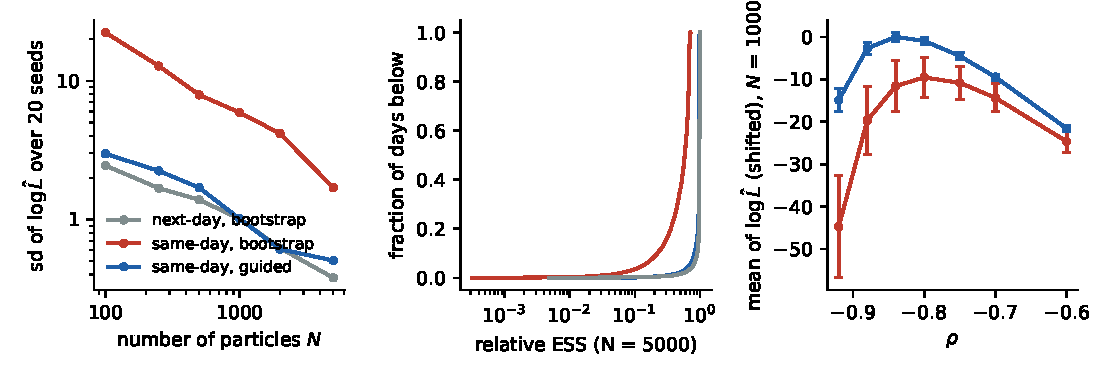
\includegraphics[width=\textwidth]{figures/pf_efficiency.pdf}
        \caption{Bootstrap and guided filters for model (iii), with the bootstrap filter for model (ii) as reference. Left: standard deviation of $\log\hat L$ on the training period over 20 random number streams. Middle: distribution of the relative ESS over all 5358 days, $N = 5000$. Right: mean $\pm$ one standard deviation of $\log\hat L$ as a function of $\rho$, the other parameters fixed at the estimate of model (iii), $N = 1000$; the curves are shifted by a common constant.}
        \label{fig:pf}
\end{figure}

\section{Parameter Estimation by Simulated Likelihood}
\label{sec:estimation}

For each model, $\hat\theta$ maximizes $\log\hat L(\theta)$ on the training period with $N = 1000$ particles and a fixed stream of random numbers (common random numbers across $\theta$). We optimize over $(10^3 a, \mu, \tanh^{-1}\phi, \log\sigma_X, \tanh^{-1}\rho)$ with Powell's method, started from the best point of a grid over $\phi$, $\sigma_X$ and $\rho$, with $\mu$ set so that the stationary variance matches the sample variance. Each model is estimated with three random number streams; each estimate is then re-evaluated with $N = 5000$ and four fresh streams, and the best is reported in Table~\ref{tab:est}. The three streams give nearly the same estimate: for model (iii), $\hat\phi$ varies by $0.0005$, $\hat\sigma_X$ by $0.002$ and $\hat\rho$ by $0.0025$. The GARCH models are fitted by maximizing their exact Gaussian likelihood.

\begin{table}[t]
        \centering
        \small
        \caption{Estimates on the training period 2000--2015. Par.: number of parameters. The log-likelihood of the SV models is the mean of four particle estimates with $N = 5000$ (standard deviation below 0.7). The last row estimates model (iii) with the bootstrap filter and evaluates the estimate with the guided filter. GJR-GARCH: $\hat\alpha \approx 0$, $\hat\gamma = 0.17$, $\hat\beta = 0.89$; GARCH: $\hat\alpha = 0.096$, $\hat\beta = 0.89$.}
        \label{tab:est}
        \begin{tabular}{lrrrrrrr}
                \toprule
                model & $10^4\hat a$ & $\hat\mu$ & $\hat\phi$ & $\hat\sigma_X$ & $\hat\rho$ & par. & log-lik. \\
                \midrule
                (i) no correlation & 5.78 & $-9.43$ & 0.983 & 0.175 & 0 & 4 & 13024.9 \\
                (ii) next-day & 1.43 & $-9.51$ & 0.977 & 0.209 & $-0.795$ & 5 & 13117.2 \\
                (iii) same-day & 5.77 & $-9.33$ & 0.987 & 0.195 & $-0.838$ & 5 & 13141.6 \\
                (iii), bootstrap estimate & 5.98 & $-9.35$ & 0.986 & 0.195 & $-0.797$ & 5 & 13140.5 \\
                GARCH(1,1) & & & & & & 4 & 12981.6 \\
                GJR-GARCH(1,1) & & & & & & 5 & 13072.5 \\
                \bottomrule
        \end{tabular}
\end{table}

All three SV models find highly persistent volatility, $\hat\phi$ between 0.977 and 0.987 (half-lives of 30 to 53 days), and a long-run daily volatility $e^{\hat\mu/2}$ of about 0.9\%. Both correlated models estimate $\rho$ near $-0.8$. In the training likelihood, model (iii) is ahead of model (ii) by 24, of GJR-GARCH by 69 and of model (i) by 117; models (ii), (iii) and GJR-GARCH have one parameter more than the other two. The training period alone therefore selects model (iii).

The estimates of $a$ differ because $a$ plays different roles. In model (i) it is the conditional mean of $R_j$, and the likelihood estimates it by, approximately, a precision-weighted average of the returns that gives calm days more weight. Calm days were mostly up days: the average of the training returns weighted by $1/\mathrm{RV}_j$ is $8.5 \times 10^{-4}$, against a plain average of $0.58 \times 10^{-4}$. In model (ii), $a$ also enters the volatility equation through $\eta_j$. In model (iii) the one-day predictive mean is not $a$ but
\[
        \Expect[R_j \mid r_{1:j-1}] = a + \rho\,\frac{\sigma_X}{2}\,\Expect\big[e^{X_j/2} \mid r_{1:j-1}\big],
\]
since $X_j = m_j + \sigma_X\xi_j$ gives $\Expect[e^{X_j/2}\xi_j \mid X_{j-1}] = \frac{\sigma_X}{2}\Expect[e^{X_j/2} \mid X_{j-1}]$. With $\hat\rho < 0$ it lies below $\hat a$: averaged over the training period it is $-2.5 \times 10^{-4}$, against $\hat a = 5.8 \times 10^{-4}$ and an average return of $0.58 \times 10^{-4}$ (standard error $1.9 \times 10^{-4}$).

\paragraph{The bias of the bootstrap objective.} Estimating model (iii) with the bootstrap filter gives $\hat\rho$ between $-0.791$ and $-0.797$ for the three streams, against $-0.84$ with the guided filter, and an estimate whose training log-likelihood is lower by 1.0. Figure~\ref{fig:pf} (right) shows why. The standard deviation of the bootstrap $\log\hat L$ grows with $|\rho|$, from 2.6 at $\rho = -0.6$ to 12 at $\rho = -0.92$, and with it the downward bias $s^2/2$, so the expected bootstrap objective peaks at a smaller $|\rho|$ than the likelihood. Common random numbers remove the noise in differences between nearby parameter values but not this bias, which itself depends on $\theta$. The guided objective has standard deviation below 1.5 down to $\rho = -0.88$, and its maximum is at $\rho = -0.84$, the estimate.

\section{One-Step Forecasts on the Held-Out Period}
\label{sec:forecasts}

All parameters are fixed at their training estimates, and the filters are run over all 5358 days with $N = 5000$; the forecast for day $j$ uses $r_{1:j-1}$ only. On the 1343 held-out days we report the predictive log-likelihood $\sum_j \log\hat p(r_j \mid r_{1:j-1})$, which scores the whole forecast distribution; the frequencies with which the probability integral transform $u_j = \hat P(R_j \le r_j \mid r_{1:j-1})$ falls in the 1\% tails \cite{dieboldGuntherTay1998}; and the QLIKE loss $\mathrm{RV}_j/h_j - \log(\mathrm{RV}_j/h_j) - 1$ of the variance forecast $h_j = \hat\Expect[e^{X_j} \mid r_{1:j-1}]$ (or the GARCH $h_j$) against the realized variance, which ranks forecasts consistently even though RV is a noisy measure of the true variance \cite{patton2011}. Differences between models are tested with $t$ statistics of the daily score differences \cite{dieboldMariano1995}.

\begin{table}[t]
        \centering
        \small
        \caption{One-step forecasts on 2016-01-04 to 2021-05-18 (1343 days). ``Gain'': predictive log-likelihood of model (iii) minus that of the row, with the $t$ statistic. PIT columns: share of days with $u_j < 0.01$, $u_j > 0.99$, and beyond three standard deviations ($\Phi^{-1}(u_j) \notin [-3, 3]$, nominal 0.27\%). QLIKE: smaller is better.}
        \label{tab:fc}
        \begin{tabular}{lrrrrrr}
                \toprule
                model & log-lik. & gain of (iii) & $u < 1\%$ & $u > 99\%$ & ${>}3$ sd & QLIKE \\
                \midrule
                (i) no correlation & 4886.4 & 22.0 ($t = 2.0$) & 1.94\% & 0.45\% & 0.82\% & 0.319 \\
                (ii) next-day & 4880.7 & 27.8 ($t = 3.1$) & 1.86\% & 0.22\% & 0.89\% & 0.334 \\
                (iii) same-day & 4908.5 & & 1.41\% & 1.04\% & 0.82\% & 0.344 \\
                GARCH(1,1) & 4798.0 & 110.5 ($t = 5.7$) & 2.08\% & 0.37\% & 1.04\% & 0.363 \\
                GJR-GARCH(1,1) & 4803.5 & 105.0 ($t = 5.5$) & 1.56\% & 0.22\% & 0.89\% & 0.362 \\
                \bottomrule
        \end{tabular}
\end{table}

\paragraph{Forecast distributions.} Model (iii) gives the best forecast distributions (Table~\ref{tab:fc}). It is ahead of model (i) by 22.0 ($t = 2.0$) and of model (ii) by 27.8 ($t = 3.1$), and the gain over model (i) is positive in 21 of the 22 years, the exception being 2017 (Figure~\ref{fig:years}). Its tail frequencies are close to the nominal 1\% on both sides, whereas all other models put too many days in the left tail and too few in the right. That asymmetry is what model (iii) builds into the one-day distribution and models (i), (ii) and the GARCH models cannot. The leverage model (ii) improves the training fit over model (i) by 92 but not the held-out forecasts, consistent with the vanishing of the next-day correlation after 2015 noted in Section 2.2. All SV models are far ahead of both GARCH models, by more than 75, although GJR-GARCH fits the training period better than model (i). The SV forecast for day $j$ is a mixture of normal distributions over the uncertain $X_j$, with heavier tails than the single normal of GARCH, and the held-out period contains large surprises.

\paragraph{Variance forecasts.} QLIKE ranks the models differently. Model (iii) beats both GARCH models ($t = 1.6$ and $1.8$), but model (i) has the lowest loss ($0.319$ against $0.344$, $t = -2.4$), although on the training period model (iii) has the lower loss by $0.020$. The held-out difference comes from the reaction to large moves. After a day whose return is more than one RV standard deviation below zero, the variance forecast of model (iii) is on average 12\% higher than that of model (i); after a day more than one standard deviation above zero, it is 13\% lower. The realized variance of 2016--2021 followed neither reaction, most visibly in 2017 and 2020 (Figure~\ref{fig:vol}, bottom). A better forecast distribution and a better variance forecast are different goals, and here they favor different models.

\paragraph{What remains.} Even for model (iii), 0.82\% of the held-out days lie beyond three predictive standard deviations, three times the nominal rate. These are days like 2018-02-05, when RV rose from 0.84\% to 2.13\% within a day while every model forecast a volatility below 0.9\%: jumps in volatility that a Gaussian AR(1) for $X_j$ does not anticipate.

\begin{figure}[t]
        \centering
        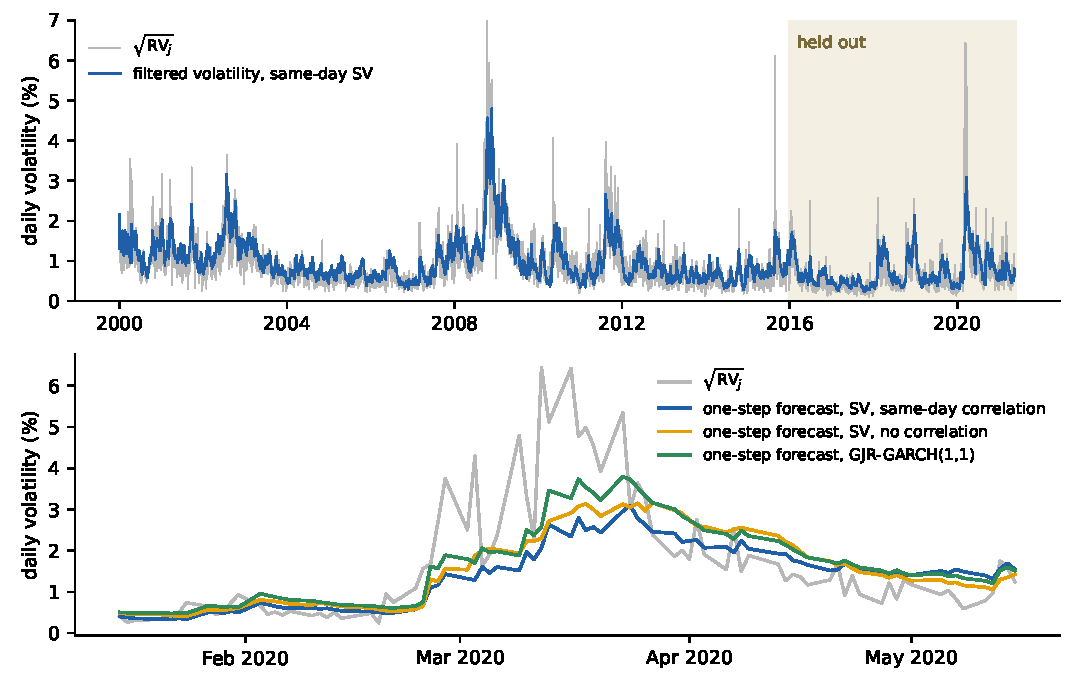
\includegraphics[width=\textwidth]{figures/volatility.pdf}
        \caption{Top: filtered volatility $\hat\Expect[e^{X_j/2} \mid r_{1:j}]$ of model (iii) and $\sqrt{\mathrm{RV}_j}$, which is not used by the filter. Bottom: one-step volatility forecasts $\sqrt{h_j}$ around the 2020 crash.}
        \label{fig:vol}
\end{figure}

\begin{figure}[t]
        \centering
        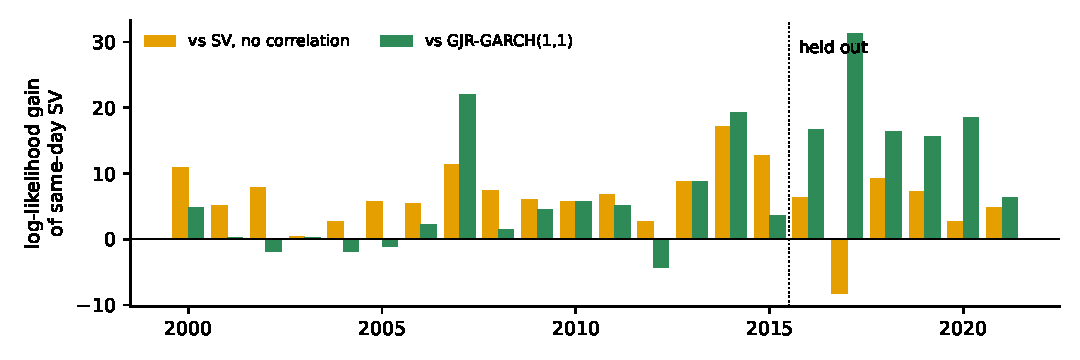
\includegraphics[width=\textwidth]{figures/gain_by_year.pdf}
        \caption{Predictive log-likelihood of model (iii) minus that of model (i) and of GJR-GARCH, by year. Parameters are estimated on 2000--2015.}
        \label{fig:years}
\end{figure}

\section{Discussion and Bibliography}

Allowing the return and the volatility to move together on the same day improves the forecast distributions of a basic SV model for the S\&P 500 out of sample, while the classical next-day leverage specification improves only the in-sample fit. Computationally, the better model is the harder one for the bootstrap particle filter. Because the same-day observation is nearly a linear Gaussian observation of the volatility shock, the optimal particle filter of Section 9.3 of the notes supplies a guided proposal almost for free. It reduces the variance of the log-likelihood estimate by a factor of 12 to 56, depending on $N$, and it removes a bias of the simulated maximum likelihood estimate of $\rho$ that common random numbers cannot remove.

Several limitations remain. Parameters are point estimates, and their uncertainty is ignored. Particle Markov chain Monte Carlo \cite{andrieuEtAl2010} would sample $\theta$ with the same unbiased likelihood estimate, and its efficiency is governed by the variance of $\log\hat L$ \cite{doucetEtAl2015}, which is where the guided proposal helps most. There is one split into training and held-out periods. The guided proposal relies on $\sigma_X$ being small, which holds here ($\hat\sigma_X \approx 0.2$); a Laplace approximation of the optimal kernel around the mode of $P(\xi_j \mid X_{j-1}, R_j)$ would remove the overshoot on extreme days and would be needed for larger $\sigma_X$. Finally, the extreme tails call for jumps in volatility rather than for heavier-tailed return shocks.

The SV model with independent shocks and its likelihood-based estimation are treated in \cite{kimShephardChib1998}. The next-day leverage specification is the Euler discretization of continuous-time SV with leverage \cite{harveyShephard1996, yu2005}; efficient MCMC for it is developed in \cite{omoriEtAl2007}. The same-day specification is that of \cite{jacquierPolsonRossi2004}, and \cite{yu2005} compares the two. The bootstrap particle filter goes back to \cite{gordonEtAl1993}; general treatments of sequential Monte Carlo and its proposals are \cite{doucetGodsillAndrieu2000, delMoral2004, chopinPapaspiliopoulos2020}, and the auxiliary particle filter \cite{pittShephard1999} is another way to use the current observation, by resampling with a predictive weight before propagating. Simulated maximum likelihood with particle filters, including resampling schemes that make $\log\hat L(\theta)$ continuous, is developed for SV models in \cite{malikPitt2011, pittMalikDoucet2014}. Forecasts are evaluated as in \cite{dieboldMariano1995, dieboldGuntherTay1998, patton2011}, and the realized measures come from \cite{heberEtAl2009}. The GARCH benchmarks are those of \cite{bollerslev1986, glostenEtAl1993}.
